%% LyX 2.0.3 created this file.  For more info, see http://www.lyx.org/.
%% Do not edit unless you really know what you are doing.
\documentclass{article}
\usepackage{graphicx, color}
\IfFileExists{upquote.sty}{\usepackage{upquote}}{}
\definecolor{fgcolor}{rgb}{0.267, 0.267, 0.267}
\newcommand{\hlnumber}[1]{\textcolor[rgb]{0,0,0}{#1}}%
\newcommand{\hlfunctioncall}[1]{\textcolor[rgb]{0.501960784313725,0,0.329411764705882}{\textbf{#1}}}%
\newcommand{\hlstring}[1]{\textcolor[rgb]{0.6,0.6,1}{#1}}%
\newcommand{\hlkeyword}[1]{\textcolor[rgb]{0,0,0}{\textbf{#1}}}%
\newcommand{\hlargument}[1]{\textcolor[rgb]{0.690196078431373,0.250980392156863,0.0196078431372549}{#1}}%
\newcommand{\hlcomment}[1]{\textcolor[rgb]{0.180392156862745,0.6,0.341176470588235}{#1}}%
\newcommand{\hlroxygencomment}[1]{\textcolor[rgb]{0.43921568627451,0.47843137254902,0.701960784313725}{#1}}%
\newcommand{\hlformalargs}[1]{\textcolor[rgb]{0.690196078431373,0.250980392156863,0.0196078431372549}{#1}}%
\newcommand{\hleqformalargs}[1]{\textcolor[rgb]{0.690196078431373,0.250980392156863,0.0196078431372549}{#1}}%
\newcommand{\hlassignement}[1]{\textcolor[rgb]{0,0,0}{\textbf{#1}}}%
\newcommand{\hlpackage}[1]{\textcolor[rgb]{0.588235294117647,0.709803921568627,0.145098039215686}{#1}}%
\newcommand{\hlslot}[1]{\textit{#1}}%
\newcommand{\hlsymbol}[1]{\textcolor[rgb]{0,0,0}{#1}}%
\newcommand{\hlprompt}[1]{\textcolor[rgb]{0.266666666666667,0.266666666666667,0.266666666666667}{#1}}%

\usepackage{color}%
 
\newsavebox{\hlnormalsizeboxclosebrace}%
\newsavebox{\hlnormalsizeboxopenbrace}%
\newsavebox{\hlnormalsizeboxbackslash}%
\newsavebox{\hlnormalsizeboxlessthan}%
\newsavebox{\hlnormalsizeboxgreaterthan}%
\newsavebox{\hlnormalsizeboxdollar}%
\newsavebox{\hlnormalsizeboxunderscore}%
\newsavebox{\hlnormalsizeboxand}%
\newsavebox{\hlnormalsizeboxhash}%
\newsavebox{\hlnormalsizeboxat}%
\newsavebox{\hlnormalsizeboxpercent}% 
\newsavebox{\hlnormalsizeboxhat}%
\newsavebox{\hlnormalsizeboxsinglequote}%
\newsavebox{\hlnormalsizeboxbacktick}%

\setbox\hlnormalsizeboxopenbrace=\hbox{\begin{normalsize}\verb.{.\end{normalsize}}%
\setbox\hlnormalsizeboxclosebrace=\hbox{\begin{normalsize}\verb.}.\end{normalsize}}%
\setbox\hlnormalsizeboxlessthan=\hbox{\begin{normalsize}\verb.<.\end{normalsize}}%
\setbox\hlnormalsizeboxdollar=\hbox{\begin{normalsize}\verb.$.\end{normalsize}}%
\setbox\hlnormalsizeboxunderscore=\hbox{\begin{normalsize}\verb._.\end{normalsize}}%
\setbox\hlnormalsizeboxand=\hbox{\begin{normalsize}\verb.&.\end{normalsize}}%
\setbox\hlnormalsizeboxhash=\hbox{\begin{normalsize}\verb.#.\end{normalsize}}%
\setbox\hlnormalsizeboxat=\hbox{\begin{normalsize}\verb.@.\end{normalsize}}%
\setbox\hlnormalsizeboxbackslash=\hbox{\begin{normalsize}\verb.\.\end{normalsize}}%
\setbox\hlnormalsizeboxgreaterthan=\hbox{\begin{normalsize}\verb.>.\end{normalsize}}%
\setbox\hlnormalsizeboxpercent=\hbox{\begin{normalsize}\verb.%.\end{normalsize}}%
\setbox\hlnormalsizeboxhat=\hbox{\begin{normalsize}\verb.^.\end{normalsize}}%
\setbox\hlnormalsizeboxsinglequote=\hbox{\begin{normalsize}\verb.'.\end{normalsize}}%
\setbox\hlnormalsizeboxbacktick=\hbox{\begin{normalsize}\verb.`.\end{normalsize}}%
\setbox\hlnormalsizeboxhat=\hbox{\begin{normalsize}\verb.^.\end{normalsize}}%



\newsavebox{\hltinyboxclosebrace}%
\newsavebox{\hltinyboxopenbrace}%
\newsavebox{\hltinyboxbackslash}%
\newsavebox{\hltinyboxlessthan}%
\newsavebox{\hltinyboxgreaterthan}%
\newsavebox{\hltinyboxdollar}%
\newsavebox{\hltinyboxunderscore}%
\newsavebox{\hltinyboxand}%
\newsavebox{\hltinyboxhash}%
\newsavebox{\hltinyboxat}%
\newsavebox{\hltinyboxpercent}% 
\newsavebox{\hltinyboxhat}%
\newsavebox{\hltinyboxsinglequote}%
\newsavebox{\hltinyboxbacktick}%

\setbox\hltinyboxopenbrace=\hbox{\begin{tiny}\verb.{.\end{tiny}}%
\setbox\hltinyboxclosebrace=\hbox{\begin{tiny}\verb.}.\end{tiny}}%
\setbox\hltinyboxlessthan=\hbox{\begin{tiny}\verb.<.\end{tiny}}%
\setbox\hltinyboxdollar=\hbox{\begin{tiny}\verb.$.\end{tiny}}%
\setbox\hltinyboxunderscore=\hbox{\begin{tiny}\verb._.\end{tiny}}%
\setbox\hltinyboxand=\hbox{\begin{tiny}\verb.&.\end{tiny}}%
\setbox\hltinyboxhash=\hbox{\begin{tiny}\verb.#.\end{tiny}}%
\setbox\hltinyboxat=\hbox{\begin{tiny}\verb.@.\end{tiny}}%
\setbox\hltinyboxbackslash=\hbox{\begin{tiny}\verb.\.\end{tiny}}%
\setbox\hltinyboxgreaterthan=\hbox{\begin{tiny}\verb.>.\end{tiny}}%
\setbox\hltinyboxpercent=\hbox{\begin{tiny}\verb.%.\end{tiny}}%
\setbox\hltinyboxhat=\hbox{\begin{tiny}\verb.^.\end{tiny}}%
\setbox\hltinyboxsinglequote=\hbox{\begin{tiny}\verb.'.\end{tiny}}%
\setbox\hltinyboxbacktick=\hbox{\begin{tiny}\verb.`.\end{tiny}}%
\setbox\hltinyboxhat=\hbox{\begin{tiny}\verb.^.\end{tiny}}%



\newsavebox{\hlscriptsizeboxclosebrace}%
\newsavebox{\hlscriptsizeboxopenbrace}%
\newsavebox{\hlscriptsizeboxbackslash}%
\newsavebox{\hlscriptsizeboxlessthan}%
\newsavebox{\hlscriptsizeboxgreaterthan}%
\newsavebox{\hlscriptsizeboxdollar}%
\newsavebox{\hlscriptsizeboxunderscore}%
\newsavebox{\hlscriptsizeboxand}%
\newsavebox{\hlscriptsizeboxhash}%
\newsavebox{\hlscriptsizeboxat}%
\newsavebox{\hlscriptsizeboxpercent}% 
\newsavebox{\hlscriptsizeboxhat}%
\newsavebox{\hlscriptsizeboxsinglequote}%
\newsavebox{\hlscriptsizeboxbacktick}%

\setbox\hlscriptsizeboxopenbrace=\hbox{\begin{scriptsize}\verb.{.\end{scriptsize}}%
\setbox\hlscriptsizeboxclosebrace=\hbox{\begin{scriptsize}\verb.}.\end{scriptsize}}%
\setbox\hlscriptsizeboxlessthan=\hbox{\begin{scriptsize}\verb.<.\end{scriptsize}}%
\setbox\hlscriptsizeboxdollar=\hbox{\begin{scriptsize}\verb.$.\end{scriptsize}}%
\setbox\hlscriptsizeboxunderscore=\hbox{\begin{scriptsize}\verb._.\end{scriptsize}}%
\setbox\hlscriptsizeboxand=\hbox{\begin{scriptsize}\verb.&.\end{scriptsize}}%
\setbox\hlscriptsizeboxhash=\hbox{\begin{scriptsize}\verb.#.\end{scriptsize}}%
\setbox\hlscriptsizeboxat=\hbox{\begin{scriptsize}\verb.@.\end{scriptsize}}%
\setbox\hlscriptsizeboxbackslash=\hbox{\begin{scriptsize}\verb.\.\end{scriptsize}}%
\setbox\hlscriptsizeboxgreaterthan=\hbox{\begin{scriptsize}\verb.>.\end{scriptsize}}%
\setbox\hlscriptsizeboxpercent=\hbox{\begin{scriptsize}\verb.%.\end{scriptsize}}%
\setbox\hlscriptsizeboxhat=\hbox{\begin{scriptsize}\verb.^.\end{scriptsize}}%
\setbox\hlscriptsizeboxsinglequote=\hbox{\begin{scriptsize}\verb.'.\end{scriptsize}}%
\setbox\hlscriptsizeboxbacktick=\hbox{\begin{scriptsize}\verb.`.\end{scriptsize}}%
\setbox\hlscriptsizeboxhat=\hbox{\begin{scriptsize}\verb.^.\end{scriptsize}}%



\newsavebox{\hlfootnotesizeboxclosebrace}%
\newsavebox{\hlfootnotesizeboxopenbrace}%
\newsavebox{\hlfootnotesizeboxbackslash}%
\newsavebox{\hlfootnotesizeboxlessthan}%
\newsavebox{\hlfootnotesizeboxgreaterthan}%
\newsavebox{\hlfootnotesizeboxdollar}%
\newsavebox{\hlfootnotesizeboxunderscore}%
\newsavebox{\hlfootnotesizeboxand}%
\newsavebox{\hlfootnotesizeboxhash}%
\newsavebox{\hlfootnotesizeboxat}%
\newsavebox{\hlfootnotesizeboxpercent}% 
\newsavebox{\hlfootnotesizeboxhat}%
\newsavebox{\hlfootnotesizeboxsinglequote}%
\newsavebox{\hlfootnotesizeboxbacktick}%

\setbox\hlfootnotesizeboxopenbrace=\hbox{\begin{footnotesize}\verb.{.\end{footnotesize}}%
\setbox\hlfootnotesizeboxclosebrace=\hbox{\begin{footnotesize}\verb.}.\end{footnotesize}}%
\setbox\hlfootnotesizeboxlessthan=\hbox{\begin{footnotesize}\verb.<.\end{footnotesize}}%
\setbox\hlfootnotesizeboxdollar=\hbox{\begin{footnotesize}\verb.$.\end{footnotesize}}%
\setbox\hlfootnotesizeboxunderscore=\hbox{\begin{footnotesize}\verb._.\end{footnotesize}}%
\setbox\hlfootnotesizeboxand=\hbox{\begin{footnotesize}\verb.&.\end{footnotesize}}%
\setbox\hlfootnotesizeboxhash=\hbox{\begin{footnotesize}\verb.#.\end{footnotesize}}%
\setbox\hlfootnotesizeboxat=\hbox{\begin{footnotesize}\verb.@.\end{footnotesize}}%
\setbox\hlfootnotesizeboxbackslash=\hbox{\begin{footnotesize}\verb.\.\end{footnotesize}}%
\setbox\hlfootnotesizeboxgreaterthan=\hbox{\begin{footnotesize}\verb.>.\end{footnotesize}}%
\setbox\hlfootnotesizeboxpercent=\hbox{\begin{footnotesize}\verb.%.\end{footnotesize}}%
\setbox\hlfootnotesizeboxhat=\hbox{\begin{footnotesize}\verb.^.\end{footnotesize}}%
\setbox\hlfootnotesizeboxsinglequote=\hbox{\begin{footnotesize}\verb.'.\end{footnotesize}}%
\setbox\hlfootnotesizeboxbacktick=\hbox{\begin{footnotesize}\verb.`.\end{footnotesize}}%
\setbox\hlfootnotesizeboxhat=\hbox{\begin{footnotesize}\verb.^.\end{footnotesize}}%



\newsavebox{\hlsmallboxclosebrace}%
\newsavebox{\hlsmallboxopenbrace}%
\newsavebox{\hlsmallboxbackslash}%
\newsavebox{\hlsmallboxlessthan}%
\newsavebox{\hlsmallboxgreaterthan}%
\newsavebox{\hlsmallboxdollar}%
\newsavebox{\hlsmallboxunderscore}%
\newsavebox{\hlsmallboxand}%
\newsavebox{\hlsmallboxhash}%
\newsavebox{\hlsmallboxat}%
\newsavebox{\hlsmallboxpercent}% 
\newsavebox{\hlsmallboxhat}%
\newsavebox{\hlsmallboxsinglequote}%
\newsavebox{\hlsmallboxbacktick}%

\setbox\hlsmallboxopenbrace=\hbox{\begin{small}\verb.{.\end{small}}%
\setbox\hlsmallboxclosebrace=\hbox{\begin{small}\verb.}.\end{small}}%
\setbox\hlsmallboxlessthan=\hbox{\begin{small}\verb.<.\end{small}}%
\setbox\hlsmallboxdollar=\hbox{\begin{small}\verb.$.\end{small}}%
\setbox\hlsmallboxunderscore=\hbox{\begin{small}\verb._.\end{small}}%
\setbox\hlsmallboxand=\hbox{\begin{small}\verb.&.\end{small}}%
\setbox\hlsmallboxhash=\hbox{\begin{small}\verb.#.\end{small}}%
\setbox\hlsmallboxat=\hbox{\begin{small}\verb.@.\end{small}}%
\setbox\hlsmallboxbackslash=\hbox{\begin{small}\verb.\.\end{small}}%
\setbox\hlsmallboxgreaterthan=\hbox{\begin{small}\verb.>.\end{small}}%
\setbox\hlsmallboxpercent=\hbox{\begin{small}\verb.%.\end{small}}%
\setbox\hlsmallboxhat=\hbox{\begin{small}\verb.^.\end{small}}%
\setbox\hlsmallboxsinglequote=\hbox{\begin{small}\verb.'.\end{small}}%
\setbox\hlsmallboxbacktick=\hbox{\begin{small}\verb.`.\end{small}}%
\setbox\hlsmallboxhat=\hbox{\begin{small}\verb.^.\end{small}}%



\newsavebox{\hllargeboxclosebrace}%
\newsavebox{\hllargeboxopenbrace}%
\newsavebox{\hllargeboxbackslash}%
\newsavebox{\hllargeboxlessthan}%
\newsavebox{\hllargeboxgreaterthan}%
\newsavebox{\hllargeboxdollar}%
\newsavebox{\hllargeboxunderscore}%
\newsavebox{\hllargeboxand}%
\newsavebox{\hllargeboxhash}%
\newsavebox{\hllargeboxat}%
\newsavebox{\hllargeboxpercent}% 
\newsavebox{\hllargeboxhat}%
\newsavebox{\hllargeboxsinglequote}%
\newsavebox{\hllargeboxbacktick}%

\setbox\hllargeboxopenbrace=\hbox{\begin{large}\verb.{.\end{large}}%
\setbox\hllargeboxclosebrace=\hbox{\begin{large}\verb.}.\end{large}}%
\setbox\hllargeboxlessthan=\hbox{\begin{large}\verb.<.\end{large}}%
\setbox\hllargeboxdollar=\hbox{\begin{large}\verb.$.\end{large}}%
\setbox\hllargeboxunderscore=\hbox{\begin{large}\verb._.\end{large}}%
\setbox\hllargeboxand=\hbox{\begin{large}\verb.&.\end{large}}%
\setbox\hllargeboxhash=\hbox{\begin{large}\verb.#.\end{large}}%
\setbox\hllargeboxat=\hbox{\begin{large}\verb.@.\end{large}}%
\setbox\hllargeboxbackslash=\hbox{\begin{large}\verb.\.\end{large}}%
\setbox\hllargeboxgreaterthan=\hbox{\begin{large}\verb.>.\end{large}}%
\setbox\hllargeboxpercent=\hbox{\begin{large}\verb.%.\end{large}}%
\setbox\hllargeboxhat=\hbox{\begin{large}\verb.^.\end{large}}%
\setbox\hllargeboxsinglequote=\hbox{\begin{large}\verb.'.\end{large}}%
\setbox\hllargeboxbacktick=\hbox{\begin{large}\verb.`.\end{large}}%
\setbox\hllargeboxhat=\hbox{\begin{large}\verb.^.\end{large}}%



\newsavebox{\hlLargeboxclosebrace}%
\newsavebox{\hlLargeboxopenbrace}%
\newsavebox{\hlLargeboxbackslash}%
\newsavebox{\hlLargeboxlessthan}%
\newsavebox{\hlLargeboxgreaterthan}%
\newsavebox{\hlLargeboxdollar}%
\newsavebox{\hlLargeboxunderscore}%
\newsavebox{\hlLargeboxand}%
\newsavebox{\hlLargeboxhash}%
\newsavebox{\hlLargeboxat}%
\newsavebox{\hlLargeboxpercent}% 
\newsavebox{\hlLargeboxhat}%
\newsavebox{\hlLargeboxsinglequote}%
\newsavebox{\hlLargeboxbacktick}%

\setbox\hlLargeboxopenbrace=\hbox{\begin{Large}\verb.{.\end{Large}}%
\setbox\hlLargeboxclosebrace=\hbox{\begin{Large}\verb.}.\end{Large}}%
\setbox\hlLargeboxlessthan=\hbox{\begin{Large}\verb.<.\end{Large}}%
\setbox\hlLargeboxdollar=\hbox{\begin{Large}\verb.$.\end{Large}}%
\setbox\hlLargeboxunderscore=\hbox{\begin{Large}\verb._.\end{Large}}%
\setbox\hlLargeboxand=\hbox{\begin{Large}\verb.&.\end{Large}}%
\setbox\hlLargeboxhash=\hbox{\begin{Large}\verb.#.\end{Large}}%
\setbox\hlLargeboxat=\hbox{\begin{Large}\verb.@.\end{Large}}%
\setbox\hlLargeboxbackslash=\hbox{\begin{Large}\verb.\.\end{Large}}%
\setbox\hlLargeboxgreaterthan=\hbox{\begin{Large}\verb.>.\end{Large}}%
\setbox\hlLargeboxpercent=\hbox{\begin{Large}\verb.%.\end{Large}}%
\setbox\hlLargeboxhat=\hbox{\begin{Large}\verb.^.\end{Large}}%
\setbox\hlLargeboxsinglequote=\hbox{\begin{Large}\verb.'.\end{Large}}%
\setbox\hlLargeboxbacktick=\hbox{\begin{Large}\verb.`.\end{Large}}%
\setbox\hlLargeboxhat=\hbox{\begin{Large}\verb.^.\end{Large}}%



\newsavebox{\hlLARGEboxclosebrace}%
\newsavebox{\hlLARGEboxopenbrace}%
\newsavebox{\hlLARGEboxbackslash}%
\newsavebox{\hlLARGEboxlessthan}%
\newsavebox{\hlLARGEboxgreaterthan}%
\newsavebox{\hlLARGEboxdollar}%
\newsavebox{\hlLARGEboxunderscore}%
\newsavebox{\hlLARGEboxand}%
\newsavebox{\hlLARGEboxhash}%
\newsavebox{\hlLARGEboxat}%
\newsavebox{\hlLARGEboxpercent}% 
\newsavebox{\hlLARGEboxhat}%
\newsavebox{\hlLARGEboxsinglequote}%
\newsavebox{\hlLARGEboxbacktick}%

\setbox\hlLARGEboxopenbrace=\hbox{\begin{LARGE}\verb.{.\end{LARGE}}%
\setbox\hlLARGEboxclosebrace=\hbox{\begin{LARGE}\verb.}.\end{LARGE}}%
\setbox\hlLARGEboxlessthan=\hbox{\begin{LARGE}\verb.<.\end{LARGE}}%
\setbox\hlLARGEboxdollar=\hbox{\begin{LARGE}\verb.$.\end{LARGE}}%
\setbox\hlLARGEboxunderscore=\hbox{\begin{LARGE}\verb._.\end{LARGE}}%
\setbox\hlLARGEboxand=\hbox{\begin{LARGE}\verb.&.\end{LARGE}}%
\setbox\hlLARGEboxhash=\hbox{\begin{LARGE}\verb.#.\end{LARGE}}%
\setbox\hlLARGEboxat=\hbox{\begin{LARGE}\verb.@.\end{LARGE}}%
\setbox\hlLARGEboxbackslash=\hbox{\begin{LARGE}\verb.\.\end{LARGE}}%
\setbox\hlLARGEboxgreaterthan=\hbox{\begin{LARGE}\verb.>.\end{LARGE}}%
\setbox\hlLARGEboxpercent=\hbox{\begin{LARGE}\verb.%.\end{LARGE}}%
\setbox\hlLARGEboxhat=\hbox{\begin{LARGE}\verb.^.\end{LARGE}}%
\setbox\hlLARGEboxsinglequote=\hbox{\begin{LARGE}\verb.'.\end{LARGE}}%
\setbox\hlLARGEboxbacktick=\hbox{\begin{LARGE}\verb.`.\end{LARGE}}%
\setbox\hlLARGEboxhat=\hbox{\begin{LARGE}\verb.^.\end{LARGE}}%



\newsavebox{\hlhugeboxclosebrace}%
\newsavebox{\hlhugeboxopenbrace}%
\newsavebox{\hlhugeboxbackslash}%
\newsavebox{\hlhugeboxlessthan}%
\newsavebox{\hlhugeboxgreaterthan}%
\newsavebox{\hlhugeboxdollar}%
\newsavebox{\hlhugeboxunderscore}%
\newsavebox{\hlhugeboxand}%
\newsavebox{\hlhugeboxhash}%
\newsavebox{\hlhugeboxat}%
\newsavebox{\hlhugeboxpercent}% 
\newsavebox{\hlhugeboxhat}%
\newsavebox{\hlhugeboxsinglequote}%
\newsavebox{\hlhugeboxbacktick}%

\setbox\hlhugeboxopenbrace=\hbox{\begin{huge}\verb.{.\end{huge}}%
\setbox\hlhugeboxclosebrace=\hbox{\begin{huge}\verb.}.\end{huge}}%
\setbox\hlhugeboxlessthan=\hbox{\begin{huge}\verb.<.\end{huge}}%
\setbox\hlhugeboxdollar=\hbox{\begin{huge}\verb.$.\end{huge}}%
\setbox\hlhugeboxunderscore=\hbox{\begin{huge}\verb._.\end{huge}}%
\setbox\hlhugeboxand=\hbox{\begin{huge}\verb.&.\end{huge}}%
\setbox\hlhugeboxhash=\hbox{\begin{huge}\verb.#.\end{huge}}%
\setbox\hlhugeboxat=\hbox{\begin{huge}\verb.@.\end{huge}}%
\setbox\hlhugeboxbackslash=\hbox{\begin{huge}\verb.\.\end{huge}}%
\setbox\hlhugeboxgreaterthan=\hbox{\begin{huge}\verb.>.\end{huge}}%
\setbox\hlhugeboxpercent=\hbox{\begin{huge}\verb.%.\end{huge}}%
\setbox\hlhugeboxhat=\hbox{\begin{huge}\verb.^.\end{huge}}%
\setbox\hlhugeboxsinglequote=\hbox{\begin{huge}\verb.'.\end{huge}}%
\setbox\hlhugeboxbacktick=\hbox{\begin{huge}\verb.`.\end{huge}}%
\setbox\hlhugeboxhat=\hbox{\begin{huge}\verb.^.\end{huge}}%



\newsavebox{\hlHugeboxclosebrace}%
\newsavebox{\hlHugeboxopenbrace}%
\newsavebox{\hlHugeboxbackslash}%
\newsavebox{\hlHugeboxlessthan}%
\newsavebox{\hlHugeboxgreaterthan}%
\newsavebox{\hlHugeboxdollar}%
\newsavebox{\hlHugeboxunderscore}%
\newsavebox{\hlHugeboxand}%
\newsavebox{\hlHugeboxhash}%
\newsavebox{\hlHugeboxat}%
\newsavebox{\hlHugeboxpercent}% 
\newsavebox{\hlHugeboxhat}%
\newsavebox{\hlHugeboxsinglequote}%
\newsavebox{\hlHugeboxbacktick}%

\setbox\hlHugeboxopenbrace=\hbox{\begin{Huge}\verb.{.\end{Huge}}%
\setbox\hlHugeboxclosebrace=\hbox{\begin{Huge}\verb.}.\end{Huge}}%
\setbox\hlHugeboxlessthan=\hbox{\begin{Huge}\verb.<.\end{Huge}}%
\setbox\hlHugeboxdollar=\hbox{\begin{Huge}\verb.$.\end{Huge}}%
\setbox\hlHugeboxunderscore=\hbox{\begin{Huge}\verb._.\end{Huge}}%
\setbox\hlHugeboxand=\hbox{\begin{Huge}\verb.&.\end{Huge}}%
\setbox\hlHugeboxhash=\hbox{\begin{Huge}\verb.#.\end{Huge}}%
\setbox\hlHugeboxat=\hbox{\begin{Huge}\verb.@.\end{Huge}}%
\setbox\hlHugeboxbackslash=\hbox{\begin{Huge}\verb.\.\end{Huge}}%
\setbox\hlHugeboxgreaterthan=\hbox{\begin{Huge}\verb.>.\end{Huge}}%
\setbox\hlHugeboxpercent=\hbox{\begin{Huge}\verb.%.\end{Huge}}%
\setbox\hlHugeboxhat=\hbox{\begin{Huge}\verb.^.\end{Huge}}%
\setbox\hlHugeboxsinglequote=\hbox{\begin{Huge}\verb.'.\end{Huge}}%
\setbox\hlHugeboxbacktick=\hbox{\begin{Huge}\verb.`.\end{Huge}}%
\setbox\hlHugeboxhat=\hbox{\begin{Huge}\verb.^.\end{Huge}}%
 

\def\urltilda{\kern -.15em\lower .7ex\hbox{\~{}}\kern .04em}%

\newcommand{\hlstd}[1]{\textcolor[rgb]{0,0,0}{#1}}%
\newcommand{\hlnum}[1]{\textcolor[rgb]{0.16,0.16,1}{#1}}
\newcommand{\hlesc}[1]{\textcolor[rgb]{1,0,1}{#1}}
\newcommand{\hlstr}[1]{\textcolor[rgb]{1,0,0}{#1}}
\newcommand{\hldstr}[1]{\textcolor[rgb]{0.51,0.51,0}{#1}}
\newcommand{\hlslc}[1]{\textcolor[rgb]{0.51,0.51,0.51}{\it{#1}}}
\newcommand{\hlcom}[1]{\textcolor[rgb]{0.51,0.51,0.51}{\it{#1}}}
\newcommand{\hldir}[1]{\textcolor[rgb]{0,0.51,0}{#1}}
\newcommand{\hlsym}[1]{\textcolor[rgb]{0,0,0}{#1}}
\newcommand{\hlline}[1]{\textcolor[rgb]{0.33,0.33,0.33}{#1}}
\newcommand{\hlkwa}[1]{\textcolor[rgb]{0,0,0}{\bf{#1}}}
\newcommand{\hlkwb}[1]{\textcolor[rgb]{0.51,0,0}{#1}}
\newcommand{\hlkwc}[1]{\textcolor[rgb]{0,0,0}{\bf{#1}}}
\newcommand{\hlkwd}[1]{\textcolor[rgb]{0,0,0.51}{#1}}


\usepackage{framed}
\makeatletter
\newenvironment{kframe}{%
 \def\FrameCommand##1{\hskip\@totalleftmargin \hskip-\fboxsep
 \colorbox{shadecolor}{##1}\hskip-\fboxsep
     % There is no \\@totalrightmargin, so:
     \hskip-\linewidth \hskip-\@totalleftmargin \hskip\columnwidth}%
 \MakeFramed {\advance\hsize-\width
   \@totalleftmargin\z@ \linewidth\hsize
   \@setminipage}}%
 {\par\unskip\endMakeFramed}
\makeatother

\definecolor{shadecolor}{rgb}{.97, .97, .97}
\newenvironment{knitrout}{}{} % an empty environment to be redefined in TeX

\usepackage[sc]{mathpazo}
\usepackage[T1]{fontenc}
\usepackage{geometry}
\usepackage[round]{natbib}
\geometry{verbose,tmargin=2.5cm,bmargin=2.5cm,lmargin=2.5cm,rmargin=2.5cm}
\setcounter{secnumdepth}{2}
\setcounter{tocdepth}{2}
\usepackage{url}
\usepackage[unicode=true,pdfusetitle,
 bookmarks=true,bookmarksnumbered=true,bookmarksopen=true,bookmarksopenlevel=2,
 breaklinks=false,pdfborder={0 0 1},backref=false,colorlinks=false]
 {hyperref}
\hypersetup{
 pdfstartview={XYZ null null 1}}
\usepackage{breakurl}
\begin{document}





\title{A Minimal Demo of glyphmaps}


\author{Garrett Grolemund}

\maketitle
This document demonstrates the basic features of the \texttt{glyphmaps} package (name may change). \texttt{glyphmaps} was written to create plots like the ones below. Each was made with \texttt{glyphmaps}. The first two plots recreate plots from \citet{wickham2011split}. The last two recreate plots from \citet{wickham2012glyph}. 













To run the examples contained in this paper, you'll have to download the \texttt{glyphmaps} development package from \url{https://github.com/garrettgman/ggplyr} and install it with

\begin{knitrout}
\definecolor{shadecolor}{rgb}{0.969, 0.969, 0.969}\color{fgcolor}\begin{kframe}
\begin{flushleft}
\ttfamily\noindent
\hlfunctioncall{library}\hlkeyword{(}\hlsymbol{devtools}\hlkeyword{)}\hspace*{\fill}\\
\hlstd{}\hlfunctioncall{load\usebox{\hlnormalsizeboxunderscore}all}\hlkeyword{(}\hlstring{"{}glyphmaps"{}}\hlkeyword{)}\mbox{}
\normalfont
\end{flushleft}
\begin{verbatim}
## Error: Can't find package glyphmaps
\end{verbatim}
\end{kframe}
\end{knitrout}


I haven't yet built the namespace or completed the documentation files, because the exact syntax / function membership hasn't been settled. As a result, the package will fail \begin{verbatim}

Error in paste(repo, branch, sep = "/", collapse = ", ") : 
  argument "repo" is missing, with no default

\end{verbatim}
.

\section{Glyphs}
The above graphs are similar in that they are all built around glyphs. I define a glyph as a geom that visually summarises information about a subset of data. Glyphs can be quite simple, or very complex. Often glyphs contain their own internal coordinate systems. The star glyphs in Figure~\ref{fig:star-glyphs} illustrate how glyphs can contain an internal (minor) coordinate system and can still be plotted in an external (major) coordinate system.




\section{glyphmaps geoms}
\texttt{glyphmaps} introduces a number of new geoms that make it easy to create glyphs. These geoms can be used in conjunction with \texttt{ggplot2} functions to create layered plots. \texttt{glyphmaps} geoms behave just like \texttt{ggplot2} geoms, but take two additional arguments, described in Section~\ref{sec:args}.










\subsection{new arguments}
\label{sec:args}
Each \texttt{glyphmaps} geom takes two new arguments, \begin{verbatim}

Error in eval(expr, envir, enclos) : object 'glyphs' not found

\end{verbatim}
 and \begin{verbatim}

Error in eval(expr, envir, enclos) : object 'reference' not found

\end{verbatim}
. \begin{verbatim}

Error in eval(expr, envir, enclos) : object 'glyphs' not found

\end{verbatim}
 controls how the data will be divided into subsets to be paired with individual glyphs. \begin{verbatim}

Error in eval(expr, envir, enclos) : object 'reference' not found

\end{verbatim}
 lets the user draw reference features with the glyphs to facilitate comparisons.

\begin{verbatim}

Error in eval(expr, envir, enclos) : object 'glyphs' not found

\end{verbatim}
 takes the name of the variable(s) to be used to divide the data into the subsets that will correspond to different glyphs. The \begin{verbatim}

Error in eval(expr, envir, enclos) : object 'glyphs' not found

\end{verbatim}
 argument works just like a \begin{verbatim}

Error in eval(expr, envir, enclos) : object '.vars' not found

\end{verbatim}
 argument in a \begin{verbatim}

Error in eval(expr, envir, enclos) : object 'ddply' not found

\end{verbatim}
 call. (In fact, the \begin{verbatim}

Error in eval(expr, envir, enclos) : object 'glyphs' not found

\end{verbatim}
 argument in a \texttt{glyphmaps} geom will be passed into a \begin{verbatim}

Error in eval(expr, envir, enclos) : object 'ddply' not found

\end{verbatim}
 call as the \begin{verbatim}

Error in eval(expr, envir, enclos) : object '.vars' not found

\end{verbatim}
 argument.)

\texttt{glyphmaps} provides methods for drawing four types of reference objects behind glyphs: boxes, vertical lines, horizontal lines, and corner points. These objects help viewers make comparisons between data inside different glyphs.







\section{Generalized glyphs}
Users are not limited to the pre-packaged glyph geoms. Any single layer plot can be turned into a glyph using the \begin{verbatim}

Error in eval(expr, envir, enclos) : object 'glyph' not found

\end{verbatim}
 and \begin{verbatim}

Error in eval(expr, envir, enclos) : object 'plyr' not found

\end{verbatim}
 functions.







The plyr function also allows users to key aesthetics to subgroups of data.




\section{Discussion - glyphs, embedded graphics, hierarchies}
Glyphs are geometric objects (i.e, geoms) designed to display information within the geom. In other words, a glyph can display information even if it is drawn by itself, without references to an external coordinate system. In reality, all geoms are a type of glyph, but the term glyph is usually reserved for complicated geoms, such as those that contain their own internal coordinate systems.

Glyphs reveal a hierarchical structure of graphics: every plot is a collection of geoms, each of which can be thought of as its own self contained plot. Sometimes these subplots are not very interesting, as in the subplot created by a single point geom. At other times, thee subplots are quite complex, as in the star glyph of Figure~\ref{fig:star-glyphs}.

Graphs inherit this hierarchical structure from the data they describe. Data is produced through an iterative process of collecting observations, grouping observations and summarizing groups of observations to create more compact, information dense sets of data. Humans innately perform this process when collecting data; it is a cognitive pattern of the human brain which I will write about in the second cognitive chapter of my thesis. 

Glyph maps simultaneously expose data from multiple levels of the hierarchy. As a set of geoms, the glyphs reveal relationships between data points in the higher level, compact data set. As individual plots, each glyph retains information about the data points in the lower level group of data that it summarises. This dual display makes glyph maps particularly useful for certain data analysis tasks. It also provides two different approaches to constructing glyph maps.

Glyph maps can be built from the top down by treating each glyph as a geom within the plot of interest. \texttt{ggplyr} provides new geoms \texttt{geom_star}, \texttt{geom_radar}, \texttt{geom_dart}, and \texttt{geom_plyr} which allow a user to quickly incorporate geoms into an existing plot.

Alternatively, glyph maps can be built from the bottom up by treating each glyph as an existing plot and then combining these plots together with an external coordinate system. This approach parallels the split-apply-combine strategy of data analysis \citep{wickham2011split}. \texttt{ggplyr} provides a set of functions such as \texttt{ggply}, \texttt{dgply}, \texttt{grid}, and \texttt{nest} that help users use the familiar split-apply-combine process to create complex glyph maps. This approach will illustrate that any graph can be turned into a glyph to be used in a higher order graph. 

The remainder of this paper will demonstrate how users can use \texttt{ggplyr} tools to build glyph maps from either the bottom up or the top down.

Although we have chosen to describe such plots as glyph maps, they really represent a general class of graphs that have been difficult to construct until now. Because each glyph is equivalent to an independent plot, glyph maps describe any plot that embeds other plots within itself. Embedded plots occur in a variety of contexts, and I have a stack of photocopies to help demonstrate this. Embedded plots also fit into the grammar of graphics, where they represent an extension of facetting. When plots are embedded into two categorical axes, a facetted plot results. When a graph is facetted on continuous axes (which is rarely done), a glyph map results. 

(Interesetingly most embedded plots have settled to the stage of embedding plots within a geographic map. This resembles how Wainer, Tufte and others have traced the development of graphs through a concrete stage where cartesian axes seldom refered to anything other than latitude and longitude. Eventually graphs became more sophisticated and axes were used to represent  abstract concepts. Perhaps embedded plots are developing through the same process, or perhaps the complexity of visualizing two orders of data at once requires one order to have a concrete interpretation.)


\section{top down methods}
\texttt{ggplyr}'s top down methods help users fit glyphs into existing methods of visualization. These methods provide new geoms (often based on new grobs) that can be used alongside existing geoms in \texttt{ggplot2}. 

Top down methods are difficult to implement in \texttt{ggplot2} for two reasons
\begin{ennumerate}
  \item First, \texttt{ggplot2} calculates aesthetics on the entire data set at once. However, glyphs contain aesthetics that must be keyed to subsets of the data.
  \item Second, the final width and height of individual glyphs often depends on non-position aesthetics, such as angle and length. In the \texttt{ggplot2} pipeline, these aesthetics are scaled right before the plot ranges are trained. As a result, the final widths of glyphs must be computed at draw time and frequently place parts of the glyph outside the plot window.
\end{ennumerate}  

\subsection{geom_plyr}
\texttt{ggplyr} provides a way for users to compute aesthetics by 



\begin{knitrout}
\definecolor{shadecolor}{rgb}{0.969, 0.969, 0.969}\color{fgcolor}\begin{kframe}
\begin{flushleft}
\ttfamily\noindent
\hlfunctioncall{set.seed}\hlkeyword{(}\hlnumber{1121}\hlkeyword{)}\hspace*{\fill}\\
\hlstd{}\hlkeyword{(}\hlsymbol{x}{\ }\hlassignement{\usebox{\hlnormalsizeboxlessthan}-}{\ }\hlfunctioncall{rnorm}\hlkeyword{(}\hlnumber{20}\hlkeyword{)}\hlkeyword{)}\mbox{}
\normalfont
\end{flushleft}
\begin{verbatim}
##  [1]  0.14496  0.43832  0.15319  1.08494  1.99954 -0.81188  0.16027  0.58589  0.36009
## [10] -0.02531  0.15088  0.11008  1.35968 -0.32699 -0.71638  1.80977  0.50840 -0.52746
## [19]  0.13272 -0.15594
\end{verbatim}
\begin{flushleft}
\ttfamily\noindent
\hlfunctioncall{mean}\hlkeyword{(}\hlsymbol{x}\hlkeyword{)}\mbox{}
\normalfont
\end{flushleft}
\begin{verbatim}
## [1] 0.3217
\end{verbatim}
\begin{flushleft}
\ttfamily\noindent
\hlfunctioncall{var}\hlkeyword{(}\hlsymbol{x}\hlkeyword{)}\mbox{}
\normalfont
\end{flushleft}
\begin{verbatim}
## [1] 0.5715
\end{verbatim}
\end{kframe}
\end{knitrout}


The first element of \texttt{x} is 0.145. Boring boxplots
and histograms recorded by the PDF device:

\begin{knitrout}
\definecolor{shadecolor}{rgb}{0.969, 0.969, 0.969}\color{fgcolor}\begin{kframe}
\begin{flushleft}
\ttfamily\noindent
\hlcomment{\usebox{\hlnormalsizeboxhash}\usebox{\hlnormalsizeboxhash}{\ }two{\ }plots{\ }side{\ }by{\ }side{\ }(option{\ }fig.show=\usebox{\hlnormalsizeboxsinglequote}hold\usebox{\hlnormalsizeboxsinglequote})}\hspace*{\fill}\\
\hlstd{}\hlfunctioncall{par}\hlkeyword{(}\hlargument{mar}{\ }\hlargument{=}{\ }\hlfunctioncall{c}\hlkeyword{(}\hlnumber{4}\hlkeyword{,}{\ }\hlnumber{4}\hlkeyword{,}{\ }\hlnumber{0.1}\hlkeyword{,}{\ }\hlnumber{0.1}\hlkeyword{)}\hlkeyword{,}{\ }\hlargument{cex.lab}{\ }\hlargument{=}{\ }\hlnumber{0.95}\hlkeyword{,}{\ }\hlargument{cex.axis}{\ }\hlargument{=}{\ }\hlnumber{0.9}\hlkeyword{,}{\ }\hlargument{mgp}{\ }\hlargument{=}{\ }\hlfunctioncall{c}\hlkeyword{(}\hlnumber{2}\hlkeyword{,}{\ }\hlnumber{0.7}\hlkeyword{,}{\ }\hlnumber{0}\hlkeyword{)}\hlkeyword{,}\hspace*{\fill}\\
\hlstd{}{\ }{\ }{\ }{\ }\hlargument{tcl}{\ }\hlargument{=}{\ }\hlkeyword{-}\hlnumber{0.3}\hlkeyword{,}{\ }\hlargument{las}{\ }\hlargument{=}{\ }\hlnumber{1}\hlkeyword{)}\hspace*{\fill}\\
\hlstd{}\hlfunctioncall{boxplot}\hlkeyword{(}\hlsymbol{x}\hlkeyword{)}\hspace*{\fill}\\
\hlstd{}\hlfunctioncall{hist}\hlkeyword{(}\hlsymbol{x}\hlkeyword{,}{\ }\hlargument{main}{\ }\hlargument{=}{\ }\hlstring{"{}"{}}\hlkeyword{)}\mbox{}
\normalfont
\end{flushleft}
\end{kframe}

{\centering 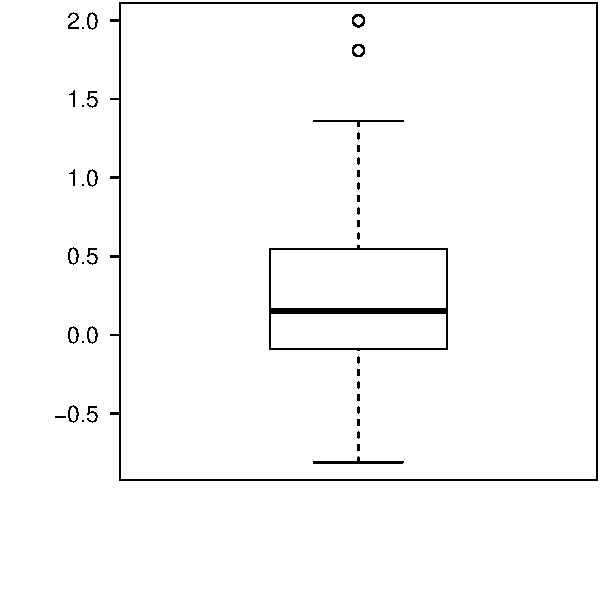
\includegraphics[width=.4\linewidth]{figure/minimal-boring-plots1} 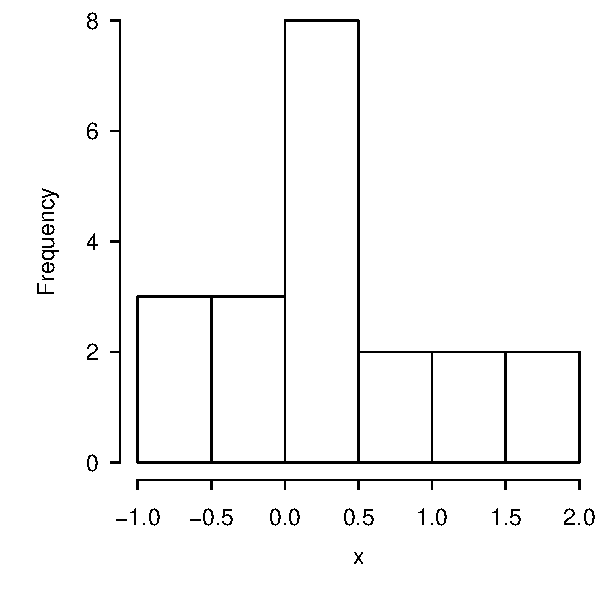
\includegraphics[width=.4\linewidth]{figure/minimal-boring-plots2} 

}


\end{knitrout}


Do the above chunks work? You should be able to compile the \TeX{}
document and get a PDF file like this one: \url{https://github.com/downloads/yihui/knitr/knitr-minimal.pdf}.
The Rnw source of this document is at \url{https://github.com/yihui/knitr/blob/master/inst/examples/knitr-minimal.Rnw}.

\bibliographystyle{plainnat}
\bibliography{ggplyr}
\end{document}
